%!TEX root = ../Report.tex


In this chapter of the report, we discuss the results of the experiments and their ramifications. The structure of this section mirrors that of the experiments section, so that the first results discussed will be the first experiment detailed in chapter \ref{chapter:experimental_methodology_and_program}.

\section{Results}
\subsection{Experiment 1}

In this experiment, the total run times of three implementations are measured. One sequential implementation, a standard modern parallel implementation utilizing OMP, and our plastic implementation. Our plastic implementation is running with no plasticity for the moment, and with no messaging functionality at all. This is so it is comparable to a standard parallel implementation.

The OMP and our implementation are using a dynamic chunks schedule, with a chunk size of 500. All programs were compiled at optimization level 3.

\begin{figure}
	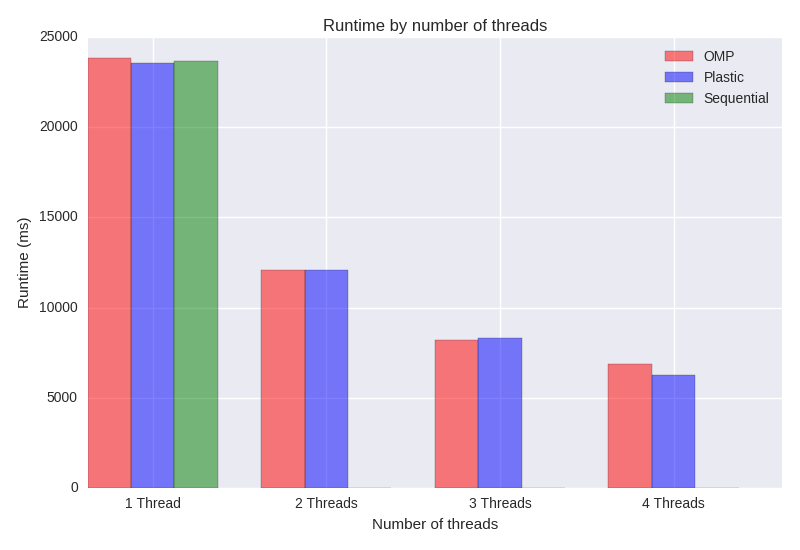
\includegraphics[width=1\textwidth]{graphics/runtime_by_number_of_threads.png}
	\caption{Total run times for an assortment of implementations and thread counts. Plastic }
	\label{fig:runtimes}
\end{figure}

Fig. \ref{fig:runtimes} shows us that with a single thread, our performance is similar to a sequential implementation, and as we increase the thread count, our performance scales accordingly. Overall, this shows that our baseline implementation performs on a par with current parallel implementations, providing a good baseline performance. 

pthread/openMP vs us(different schedules?)

pthread/openMP w/ 2threads vs us w/ 2 threads then 4 (plasticity!)       - highlights importance of parameters

pthread/openMP w/ fixed schedule vs us switching schedules (plasticity!) - highlights importance of schedule choice

 Above with skewed task distribution

\section{Discussion}

 ***Discuss the findings of the results, (Mention weird runtimes with many small tasks!)***